\documentclass{beamer}
\usepackage{graphicx}
\begin{document}
\begin{frame}
\frametitle{Resilience levels of tree growth}
\begin{figure}
% \begin{minipage}[b]{0.4\textwidth}
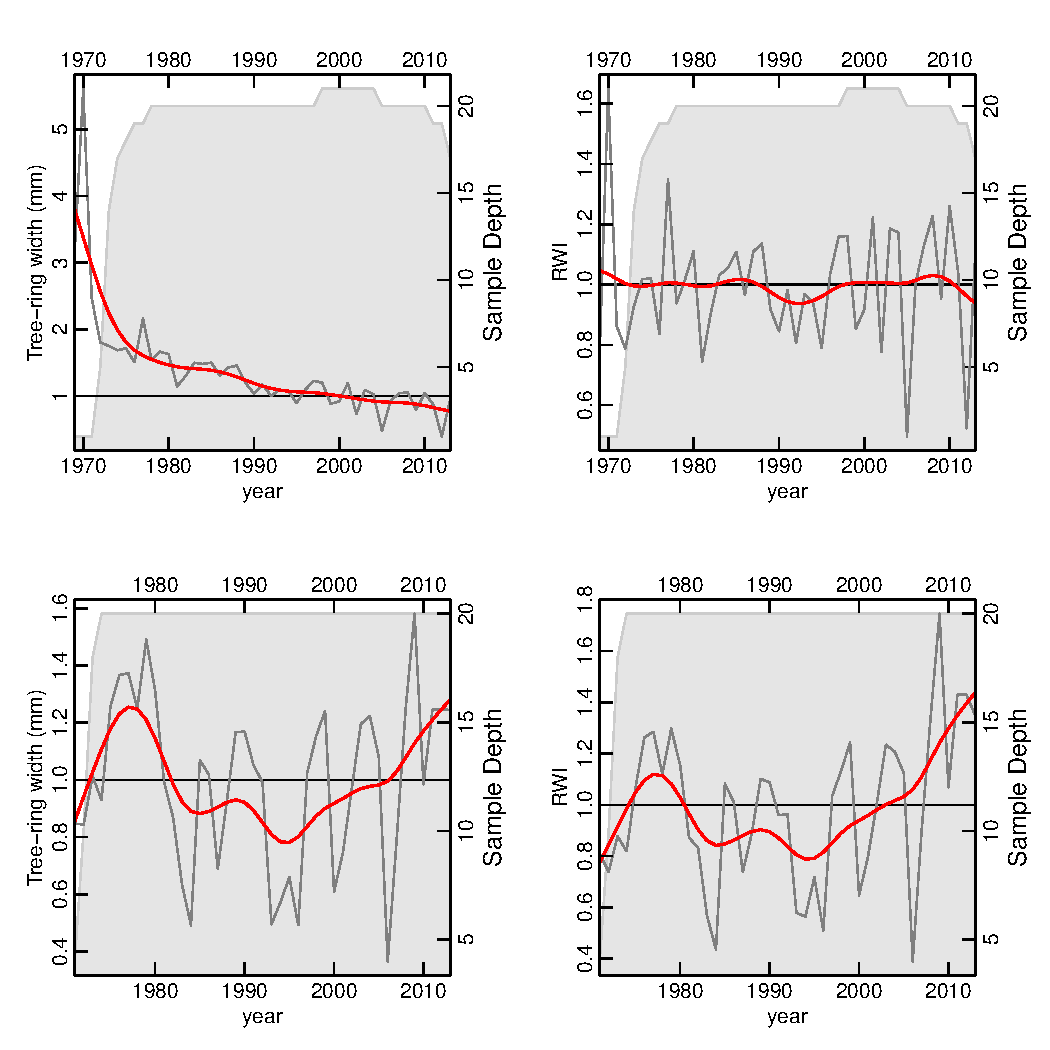
\includegraphics[width = 0.6\textwidth]{RWIs}
% \end{minipage}
\end{figure}
Tree growt in the north has high resistance but slow recovery. Tree
growth in the south has slow resistance and slow recovery.
\end{frame}

\begin{frame}
  \frametitle{Resilience levels of Isotopic concentrations}
\begin{figure}
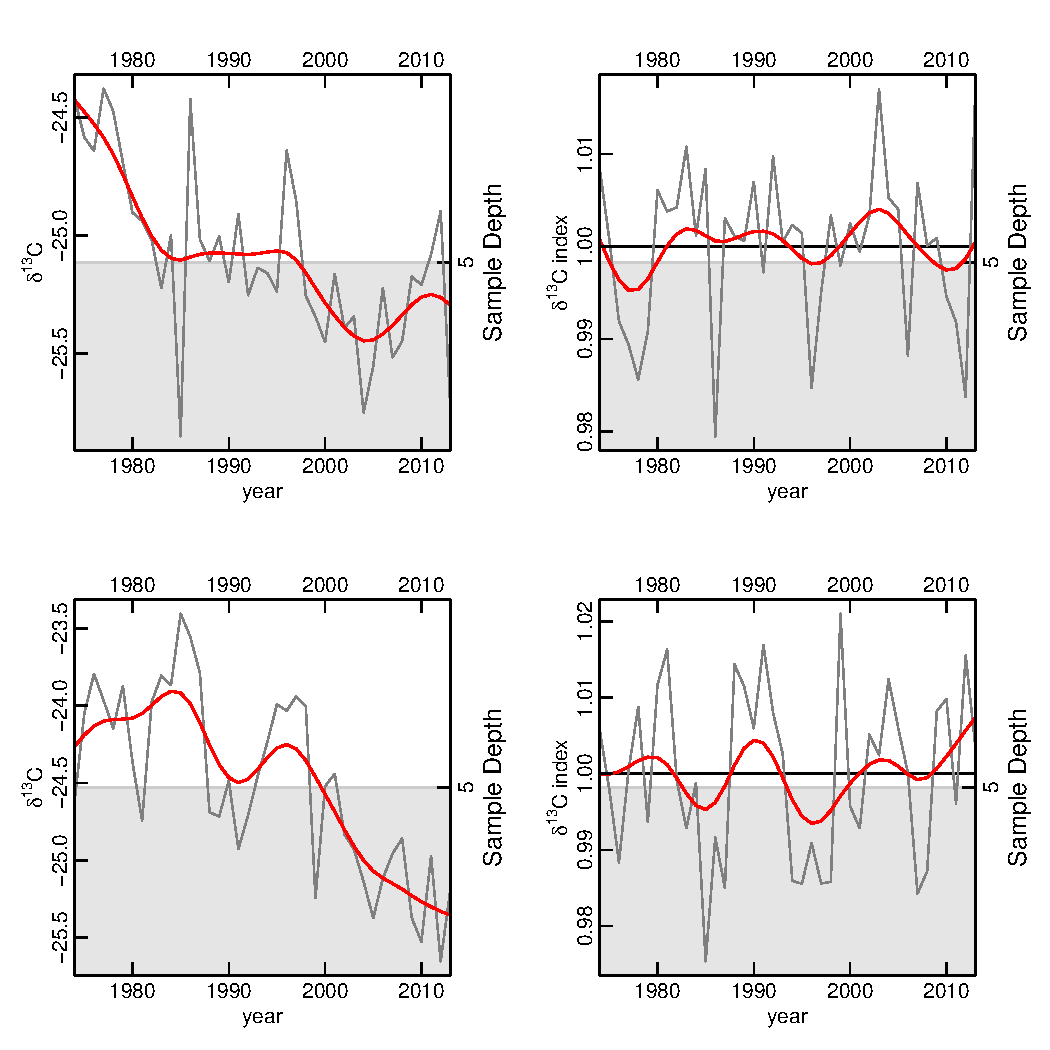
\includegraphics[width = 0.6\textwidth]{ideltas}
\end{figure}
\end{frame}

\begin{frame}
\frametitle{Cross-correlation functions}
\begin{figure}
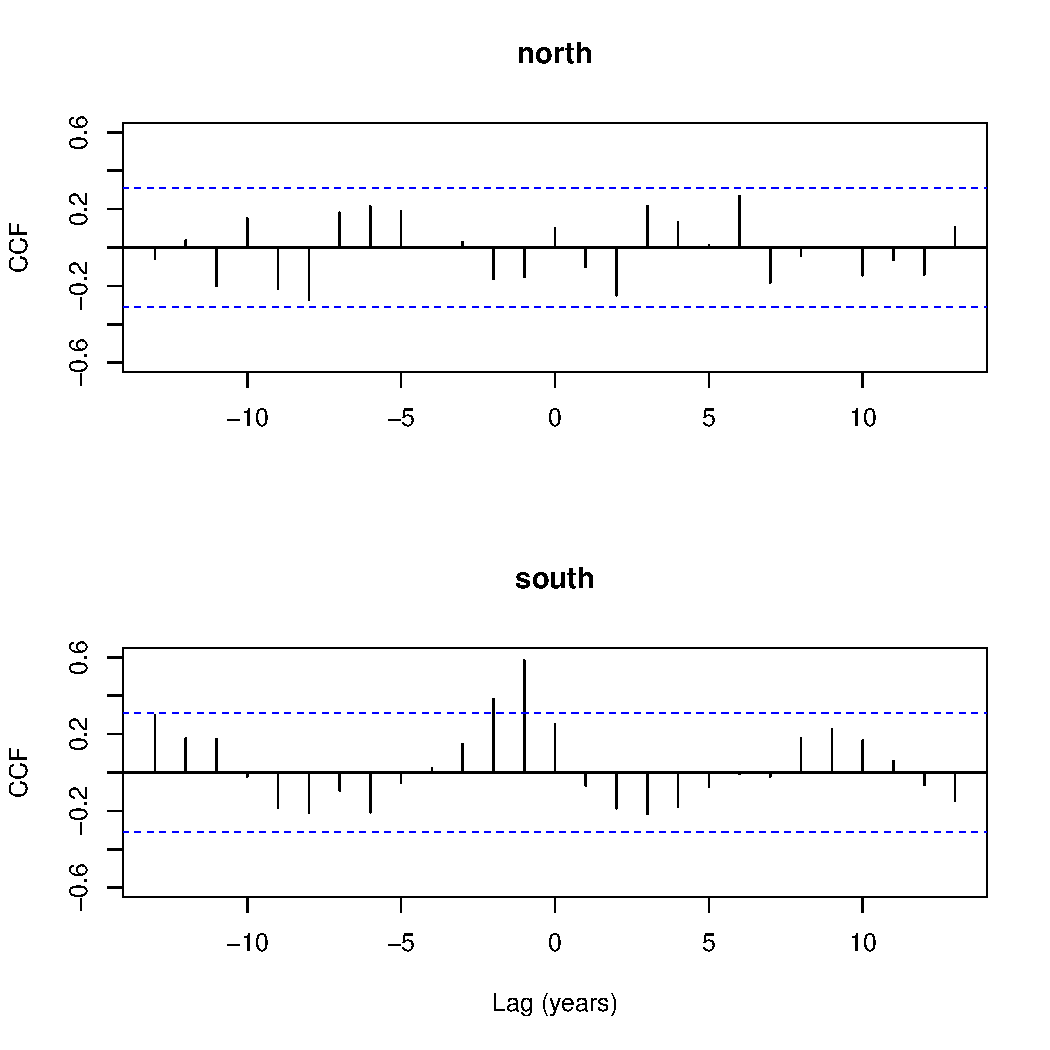
\includegraphics[width = 0.6\textwidth]{CCFFun}
\end{figure}
Annual tree growth was correlated with isotopic concentration of the
previous year (south).
\end{frame}

\begin{frame}
\frametitle{Seasonal Responses}
\begin{figure}
\begin{minipage}[b]{0.4\textwidth}
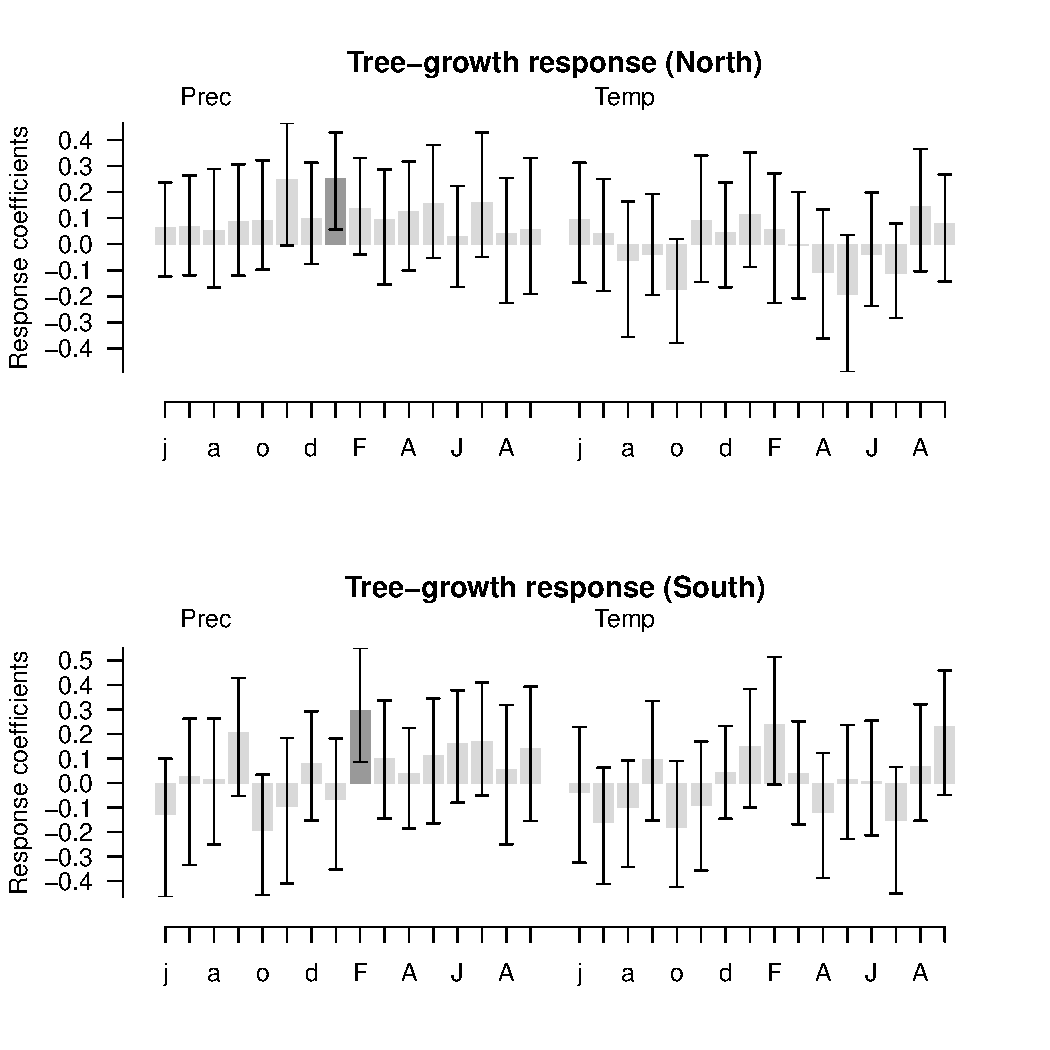
\includegraphics[width = \textwidth]{GrowthFunRes}
\end{minipage}
\begin{minipage}[b]{0.4\textwidth}
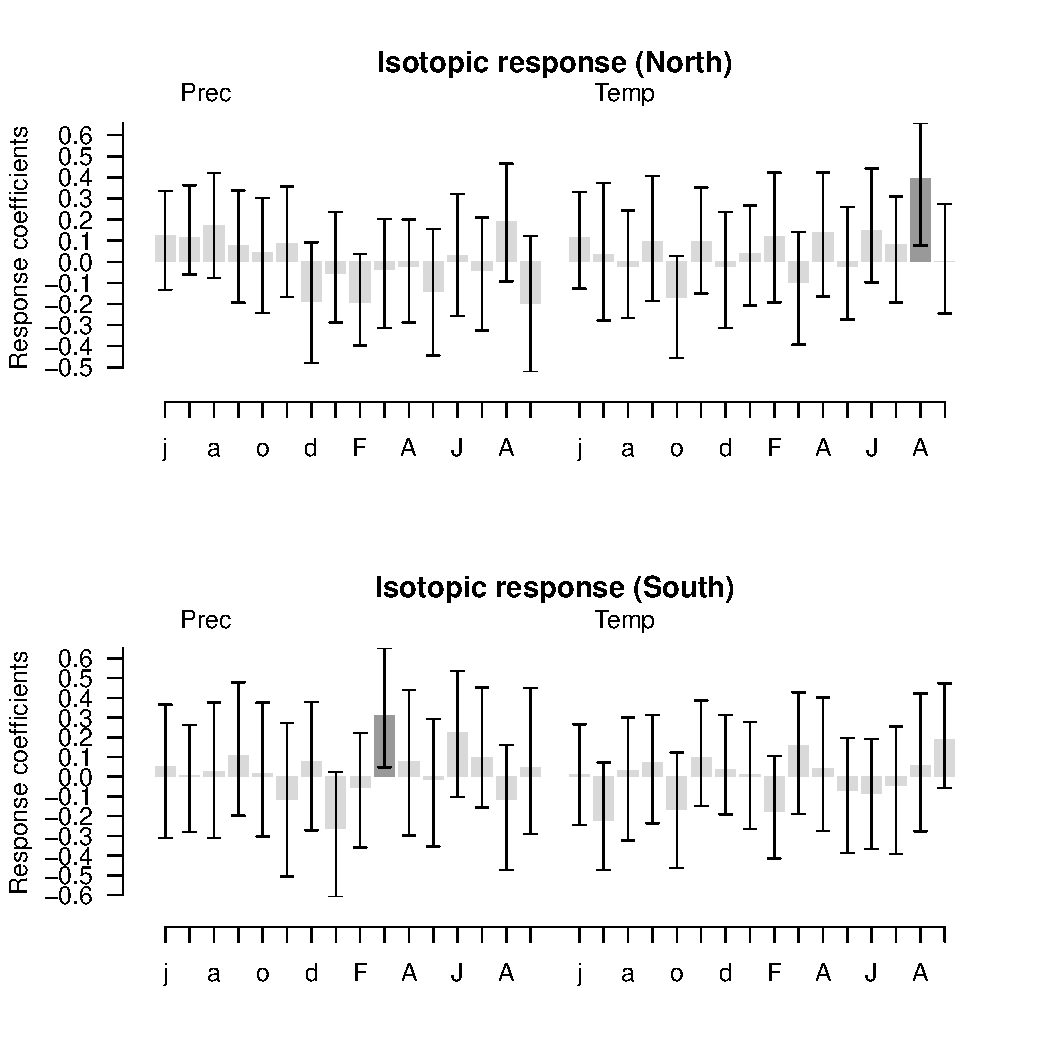
\includegraphics[width = \textwidth]{IsoFunRes}
\end{minipage}
\end{figure}
Spring moisture has a significant controlling influence on tree growth
(north and south), and on isotopic concentrations (south). Summer
temperature significantly affected isotopic concentrations (north)
\end{frame}

\begin{frame}
\frametitle{Inter-annual coherence (SPEI and tree-ring widths)}
\begin{figure}
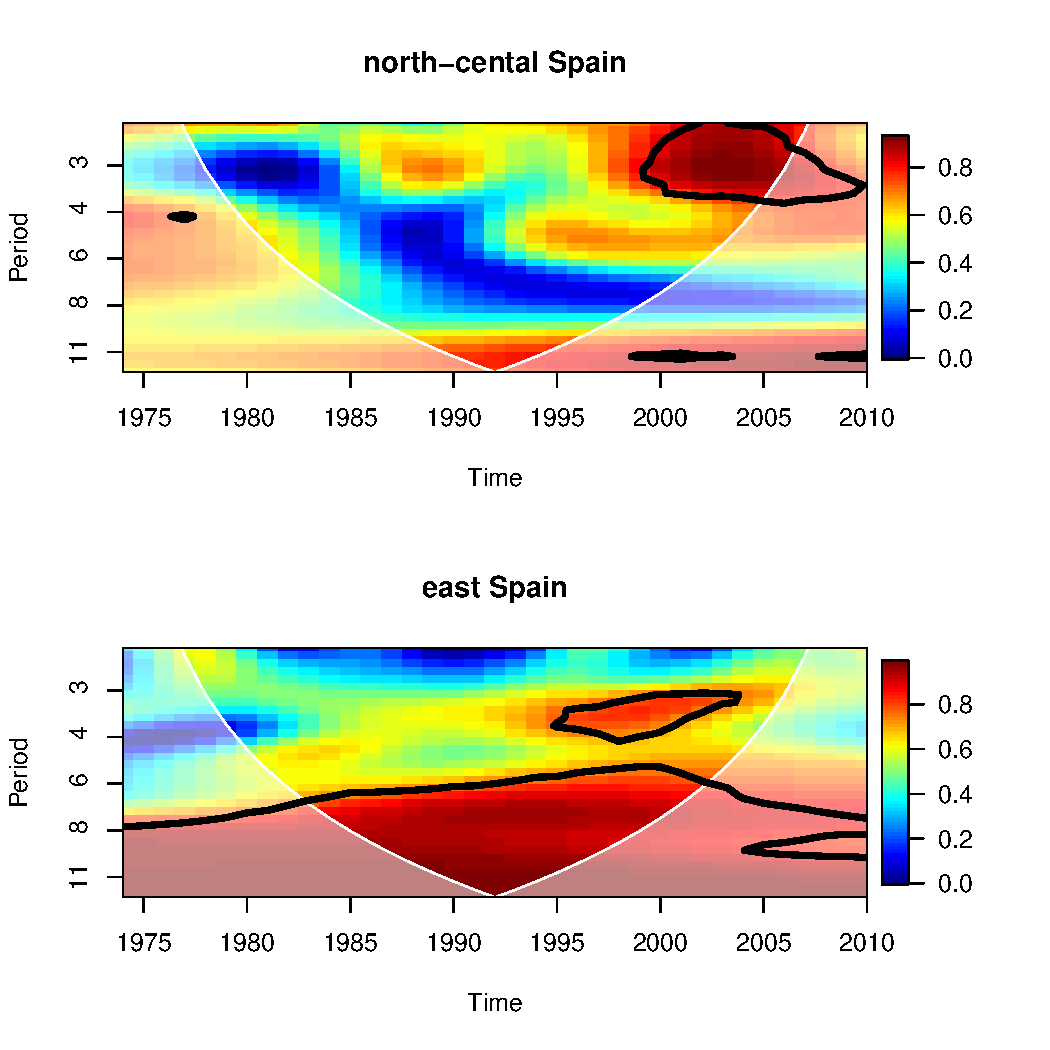
\includegraphics[width = 0.6\textwidth]{coherence1}
\end{figure}
Annual tree growth was correlated with isotopic concentration of the
previous year (south).
\end{frame}


\end{document}